%%%%%%%%%%%%%%%%%%%%%%%%%%%%%%%%%%%%%%%%%%%%%%%%%%%%%%%%%%%%%%%
%                                                             %
%    Document class                                           %
%                                                             %
%%%%%%%%%%%%%%%%%%%%%%%%%%%%%%%%%%%%%%%%%%%%%%%%%%%%%%%%%%%%%%%

\documentclass[10pt]{ltjsarticle}

%%%%%%%%%%%%%%%%%%%%%%%%%%%%%%%%%%%%%%%%%%%%%%%%%%%%%%%%%%%%%%%
%                                                             %
%    Standard packages                                        %
%                                                             %
%%%%%%%%%%%%%%%%%%%%%%%%%%%%%%%%%%%%%%%%%%%%%%%%%%%%%%%%%%%%%%%

\usepackage{amsmath}
\usepackage{amsthm}
\usepackage{enumitem}
\usepackage{graphicx}
\usepackage{tikz}
\usetikzlibrary{cd}
\usepackage{clock}
\usepackage{lipsum}

%%%%%%%%%%%%%%%%%%%%%%%%%%%%%%%%%%%%%%%%%%%%%%%%%%%%%%%%%%%%%%%
%                                                             %
%    Additional packages                                      %
%                                                             %
%%%%%%%%%%%%%%%%%%%%%%%%%%%%%%%%%%%%%%%%%%%%%%%%%%%%%%%%%%%%%%%

\usepackage{packages/rayout} % レイアウト
\usepackage{packages/math} % 数学記号等
\usepackage{packages/theorem} % 定理環境
\usepackage{packages/code} % ソースコード
\usepackage{packages/bibliography} % 参考文献
\bibliography{refs}
\usepackage{packages/hyperlink}

%%%%%%%%%%%%%%%%%%%%%%%%%%%%%%%%%%%%%%%%%%%%%%%%%%%%%%%%%%%%%%%
%                                                             %
%    Body                                                     %
%                                                             %
%%%%%%%%%%%%%%%%%%%%%%%%%%%%%%%%%%%%%%%%%%%%%%%%%%%%%%%%%%%%%%%

\title{LaTeXテンプレート}
\author{野本 慶一郎}
\date{最終更新: \today \texthours 時 \textminutes 分 \clocktime}

\begin{document}
\maketitle
\thispagestyle{plain}
\tableofcontents
\newpage

% ----------------------------------------------------------- %

\section{記号・数式}

\subsection{数学文字}

\begin{description}[labelwidth=\widthof{フラクトゥール(mathfrak)}]
	\item[黒板文字(mathbb)] $\bbA, \bbB, \bbC, \bbD, \dots$
	\item[筆記体(mathcal)] $\calA, \calB, \calC, \calD, \dots$
	\item[フラクトゥール(mathfrak)] $\frakA, \frakB, \frakC, \frakD, \dots, \fraka, \frakb, \frakc, \frakd, \dots$
	\item[花文字(mathscr)] $\scrA, \scrB, \scrC, \scrD, \dots$
\end{description}

\subsection{数学作用素}

MyMathOperatorsに登録した文字は数学作用素として書くことができる.
例えば
\begin{align}
	\Ker f, \ \Hom(\frakg, \frakh), \ \Gal(\bar{K}/K), \ \Spec A, \ \rank E(\bbQ), \ \Sel^{(\phi)}(E/K)
\end{align}
のように使用可能.

\subsection{数式}

align環境で数式を書く際には, ラベリングをするかどうかに関わらず「*」は付けなくてよい.
例えば数式
\begin{align}
	\zeta(s)\coloneqq\sum_{n=1}^{\infty}\frac{1}{n^s} \label{eq:RiemannZetaFunction}
\end{align}
は引用していないので, 式番号は付いていない. しかし
\begin{align}
	f(z_0)=\frac{1}{2\pi i}\oint_{C}\frac{f(z)}{z-z_0}dz \label{eq:CauchyIntegralFormula}
\end{align}
は式\ref{eq:CauchyIntegralFormula}と引用したので式番号が表示されている.
また, 括弧は
\begin{align}
	\skakko*{\frac{q}{p}}, \ \mkakko*{0, \frac{k}{m}}, \ \lkakko*{\frac{1}{n+1}x^{n+1}}_{x=a}^{b}
\end{align}
のように簡潔に書くことができる. また, 集合は
\begin{align}
    \set*{(a_{i})\in\prod A_i}{f_{ij}(a_j)=a_i}
\end{align}
と書くことができる.


% ----------------------------------------------------------- %
\newpage
\section{定理・コメント}

\subsection{定理環境}

定義や命題等は, 以下のようにして記述する:
\begin{defi}{群の定義{\cite[命題 hoge]{赤雪江}}}{Group}
	空でない集合$G$が\textbf{群}であるとは, 写像
	\begin{align}
		\phi: G\times G\to G
	\end{align}
	で以下の三つの条件を満たすものが存在することをいう.
	\begin{description}[labelwidth=\widthof{単位元の存在}]
		\item[結合法則] ${}^{\forall} g, h, i\in G, \ \phi(\phi(g, h), i)=\phi(g, \phi(h, i))$.
		\item[単位元の存在] ${}^{\exists} e\in G \ \text{s.t.} \ {}^{\forall} g\in G, \ \phi(g, e)=\phi(e, g)=e$.
		\item[逆元の存在] ${}^{\forall} g\in G, {}^{\exists} g^{-1}\in G \ \text{s.t.} \ \phi(g, g^{-1})=\phi(g^{-1}, g)=e$. 
	\end{description}
	$\phi(g, h)$のことを単に, $g\cdot h$や$gh$と書くことがある.
\end{defi}

\begin{prop}{単位元の一意性{\cite[命題 hoge]{赤雪江}}}{UniqueIdentityElement}
	群$G$の単位元$e$は一意的に存在する.
\end{prop}
\begin{proof}
	$e, e'\in G$を単位元とする. 定義\ref{defi:Group}より
	\begin{align}
		e
		&=e\cdot e' \quad (\because e'\text{は単位元})\\
		&=e' \quad (\because e\text{は単位元})
	\end{align}
	が成り立つ. したがって群の単位元は一意的に存在する.
\end{proof}

\begin{rem}{{\cite[命題 hoge]{赤雪江}}}{UniqueInverseElement}
	命題\ref{prop:UniqueIdentityElement}と同様にして, 逆元の一意性も証明することができる.
\end{rem}
% ----------------------------------------------------------- %
\newpage
\section{図}

準同型定理の図式は以下のようにして書ける.
\begin{align}
	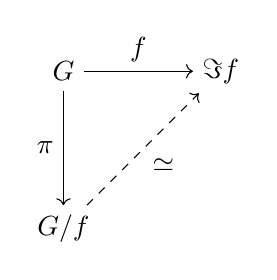
\begin{tikzpicture}[auto]
		\node (G) at (0, 2) {$G$};
		\node (Imf) at (2, 2) {$\Im f$};
		\node (GKerf) at (0, 0) {$G/\Ker f$};
		\node (Circle) at (0.6, 1.3) {$\circlearrowright$};
		\draw[->] (G) to node {$f$} (Imf);
		\draw[->] (G) to node[swap] {$\pi$} (GKerf);
		\draw[->, dashed] (GKerf) to node[swap] {$\simeq$} (Imf);
	\end{tikzpicture}
\end{align}
ファイバー積の普遍性は以下のようにして書ける.
\begin{align}
	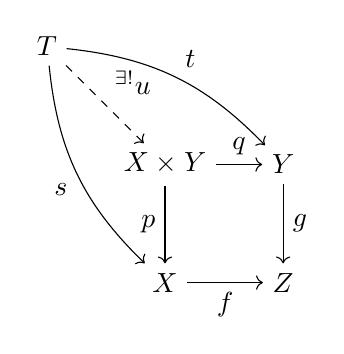
\begin{tikzpicture}[auto]
		\node (T) at (0, 3) {$T$};
		\node (X) at (1.5, 0) {$X$};
		\node (XxY) at (1.5, 1.5) {$X\times_{\bbZ}Y$};
		\node (Z) at (3, 0) {$Z$};
		\node (Y) at (3, 1.5) {$Y$};
		\draw[->, dashed] (T) to node {${}^{\exists!}u$} (XxY);
		\draw[->] (T) to[bend left=20] node {$t$} (Y);
		\draw[->] (T) to[bend right=20] node[swap] {$s$} (X);
		\draw[->] (XxY) to node {$q$} (Y);
		\draw[->] (XxY) to node[swap] {$p$} (X);
		\draw[->] (Y) to node {$g$} (Z);
		\draw[->] (X) to node[swap] {$f$} (Z);
	\end{tikzpicture}
\end{align}
% ----------------------------------------------------------- %
\newpage
\section{アルゴリズム・コード}

\subsection{疑似コード}

疑似コード例は以下のようにして書くことができる.

\begin{algorithm}

	\caption{Euclidの互除法}
	
	\begin{algorithmic}[1]

		\Function{Euclid}{$a,b$}
			\State $r\gets a\bmod b$
			\While{$r\not=0$} \Comment{$r=0$ならば最大公約数は$b$}
				\State $a\gets b$
				\State $b\gets r$
				\State $r\gets a\bmod b$
			\EndWhile
			\State \textbf{return} $b$
		\EndFunction

	\end{algorithmic}

\end{algorithm}

高速に冪乗$a^n$を計算するアルゴリズムである\red{繰り返し二乗法}を説明する.
簡単のため, 非負整数$n\in\bbZ$のサイズは高々3ビット, すなわち$n$は
\begin{align}
	n=n_0+n_12+n_22^2 \quad (n_0, n_1, n_2\in \{0, 1\})
\end{align}
という2進展開で表示されるとする. このとき
\begin{align}
	a^n
	&=a^{n_0+n_12+n_22^2}\\
	&=a^{n_0}\cdot a^{n_12+n_22^2}\\
	&=a^{n_0}\cdot \skakko*{a^{n_1+n_22}}^2\\
	&=a^{n_0}\cdot \skakko*{a^{n_1}\cdot \skakko*{a^{n_2}}^2}^2\\
	&=a^{n_0}\cdot \skakko*{a^{n_1}\cdot \skakko*{a^{n_2}\cdot \skakko*{1}^2}^2}^2\\ \label{eq:square}
\end{align}
が成り立つ. したがってこの場合は二乗算を3回, 乗算を高々3回で計算可能である.
\footnote{一般に, 繰り返し二乗法の計算量は$O(\log_2 n)$である.}
式\eqref{eq:square}に従って冪乗$a^n$を計算するアルゴリズムが繰り返し二乗法である.

\begin{algorithm}

	\caption{繰り返し二乗法}
	
	\begin{algorithmic}[1]

		\Function{pow}{$a,n$}
			\State $n=n_0+n_12+n_22^2+\dots+n_{\ell-1}2^{\ell-1}$と表す
			\State $\texttt{val}\gets 1$
			\For{$i$}{$\ell-1$}{$0$}
				\State $\texttt{val}\gets \texttt{val}\times\texttt{val}$
				\If{$n_i == 1$}
					\State $\texttt{val}\gets a\times\texttt{val}$
				\EndIf
			\EndFor
			\State \textbf{return} \texttt{val}
		\EndFunction

	\end{algorithmic}

\end{algorithm}

\subsection{ソースコード}

\lipsum[1-2]
% \begin{python}
% E = EllipticCurve([1, 0])
% r = E.rank() % あいうえお
% if r != 0: % aiueo
% 	print r
% def aiueo():
% 	return f"2={1+1}"
% \end{python}
% ----------------------------------------------------------- %

% ----------------------------------------------------------- %
\newpage
\printbibliography[title=参考文献]

\end{document}

